\documentclass[11pt,a4paper]{ctexart}

% ============ 基础宏包 ============
\usepackage[margin=2.5cm]{geometry}
\usepackage{amsmath,amssymb,amsthm,mathtools}
\usepackage{tikz}
\usetikzlibrary{trees,positioning,arrows.meta,calc,decorations.pathreplacing}
\usepackage{graphicx}
\usepackage{enumitem}
\usepackage{xcolor}
\usepackage{tcolorbox}
\tcbuselibrary{theorems,skins,breakable}
\usepackage{booktabs}
\usepackage{array}
\usepackage{caption}
\usepackage{hyperref}
\hypersetup{colorlinks=true,linkcolor=blue!60!black,urlcolor=blue!60!black,citecolor=blue!60!black}

% ============ 主题色 ============
\definecolor{mainblue}{RGB}{30,90,160}
\definecolor{lightblue}{RGB}{220,235,250}
\definecolor{accentred}{RGB}{180,50,50}
\definecolor{lightred}{RGB}{250,230,230}
\definecolor{accentgreen}{RGB}{40,120,70}
\definecolor{lightgreen}{RGB}{230,245,232}

% ============ 定理环境 ============
\newtcbtheorem[number within=section]{exmp}{例}
{enhanced,colback=lightblue,colframe=mainblue,fonttitle=\bfseries,
 breakable,attach boxed title to top left={xshift=4mm,yshift=-2.5mm},
 boxed title style={colback=mainblue,sharp corners}}{ex}

\newtcbtheorem[number within=section]{defn}{定义}
{enhanced,colback=lightgreen,colframe=accentgreen,fonttitle=\bfseries,
 breakable,attach boxed title to top left={xshift=4mm,yshift=-2.5mm},
 boxed title style={colback=accentgreen,sharp corners}}{def}

\newtcbtheorem[number within=section]{idea}{核心思想}
{enhanced,colback=lightred,colframe=accentred,fonttitle=\bfseries,
 breakable,attach boxed title to top left={xshift=4mm,yshift=-2.5mm},
 boxed title style={colback=accentred,sharp corners}}{key}

% ============ 数学符号 ============
\newcommand{\E}{\mathbb{E}}
\newcommand{\Q}{\mathbb{Q}}
\newcommand{\R}{\mathbb{R}}
\newcommand{\1}{\mathbf{1}}

% ============ 标题信息 ============
\title{\bfseries 从二叉树期权定价到强化学习\\[4pt]
       \large 用一个金融决策问题理解最优决策的数学结构}
\author{}
\date{}

\begin{document}
\maketitle

\begin{abstract}
\noindent 本讲义面向没有金融背景、也没有强化学习基础的同学。我们从一个具体的金融问题——\textbf{期权定价}——出发，用最简单的二叉树模型一步一步往前推。当推到\textbf{美式期权}时，会自然冒出一个核心问题：每一步要不要现在行权？这个看似简单的"要不要"，恰恰就是\textbf{强化学习}里"动作选择"的本质。讲义的目标是让你在读完之后，不仅会用二叉树给期权定价，更重要的是，能看穿期权定价、最优控制和强化学习\textbf{是同一套数学}。
\end{abstract}

\tableofcontents
\vspace{1em}\hrule\vspace{1em}

% ==========================================================
\section{从一个保险的故事开始}
% ==========================================================

想象你是一家航空公司的财务经理。航空公司最大的成本之一是航空燃油，而油价波动剧烈：今天每桶 80 美元，三个月后可能涨到 100，也可能跌到 60。

你怎么办？

一个办法是去找一家银行，签一份合同：

\begin{quote}
\itshape "三个月后，无论实际油价是多少，我都\textbf{有权利}以每桶 90 美元的价格向你买一桶油；但如果到时候市场价比 90 还便宜，我可以不买。"
\end{quote}

这份合同有两个特点：

\begin{itemize}[leftmargin=*]
    \item 它给了你\textbf{权利}（right），但没有给你\textbf{义务}（obligation）。如果三个月后油价是 100，你高兴地以 90 买下，省了 10 块；如果油价是 60，你直接去市场买，扔掉这份合同就行。
    \item 这份合同本身值钱。银行不会白送给你——它要收一笔费用，比如 5 美元/桶。
\end{itemize}

这就是一份\textbf{期权（option）}。我们这门课要回答的第一个问题非常具体：

\begin{idea}{这份合同应该卖多少钱？}{price-question}
\itshape 直觉是模糊的：5 美元？8 美元？凭什么？银行收太少会亏本，收太多没人买。一定有一个"公平"的价格，使得这份合同对买方和卖方都不偏不倚。这个公平价格怎么算？
\end{idea}

让人意外的是：回答这个问题，会把我们一路带到强化学习。

% ==========================================================
\section{期权的基本概念}
% ==========================================================

我们先把行话理清楚。

\subsection{底层资产、行权价、到期日}

一份期权是一份合同，它涉及以下要素：

\begin{itemize}[leftmargin=*]
    \item \textbf{底层资产（underlying）}: 这份合同"挂钩"的对象，例如某只股票、一桶原油、一吨大豆。我们用 $S_t$ 表示它在时刻 $t$ 的价格。
    \item \textbf{行权价（strike price）}: 合同中事先约定好的成交价，记作 $K$。
    \item \textbf{到期日（maturity / expiry）}: 合同的截止时刻，记作 $T$。
\end{itemize}

\subsection{看涨期权与看跌期权}

\begin{defn}{看涨与看跌}{call-put}
\textbf{看涨期权（call option）}: 合同持有人\emph{有权利}在到期日以价格 $K$ \emph{买入}一单位底层资产。到期日的收益是：
\[
\text{Call 收益} = \max(S_T - K,\, 0) =: (S_T - K)^+
\]
\textbf{看跌期权（put option）}: 合同持有人\emph{有权利}在到期日以价格 $K$ \emph{卖出}一单位底层资产。到期日的收益是：
\[
\text{Put 收益} = \max(K - S_T,\, 0) =: (K - S_T)^+
\]
\end{defn}

为什么取 $\max(\cdot, 0)$？因为持有人不会让自己亏钱。比如看涨期权，到期时如果 $S_T = 80$ 而 $K = 90$，你不可能傻到以 90 元买一个市场价 80 元的东西——你直接放弃这个权利，收益为 0。

\medskip
\noindent\textbf{术语}：把上面这条小学生都看得懂的曲线（如图~\ref{fig:payoff}）叫做期权的\emph{收益函数（payoff function）}。它是分段线性的，全部复杂性就藏在那个 $\max$ 里——这正是后面美式期权出现"决策"的根源。

\begin{figure}[h]
\centering
\begin{tikzpicture}[scale=0.9]
% Call
\begin{scope}[xshift=-5cm]
\draw[->] (0,0) -- (5.5,0) node[right] {$S_T$};
\draw[->] (0,-0.5) -- (0,3.5) node[above] {收益};
\draw[thick,mainblue] (0,0) -- (2.5,0) -- (5,2.5);
\draw[dashed] (2.5,0) -- (2.5,-0.3) node[below] {$K$};
\node at (2.5,3) {\bfseries 看涨期权 (Call)};
\node at (4.2,1.5) [right] {\small $(S_T-K)^+$};
\end{scope}
% Put
\begin{scope}[xshift=3cm]
\draw[->] (0,0) -- (5.5,0) node[right] {$S_T$};
\draw[->] (0,-0.5) -- (0,3.5) node[above] {收益};
\draw[thick,accentred] (0,2.5) -- (2.5,0) -- (5,0);
\draw[dashed] (2.5,0) -- (2.5,-0.3) node[below] {$K$};
\node at (2.5,3) {\bfseries 看跌期权 (Put)};
\node at (0.5,1.8) [right] {\small $(K-S_T)^+$};
\end{scope}
\end{tikzpicture}
\caption{看涨与看跌期权的到期收益函数。}
\label{fig:payoff}
\end{figure}

\subsection{欧式与美式}

行权时间上还有两种主要类型：

\begin{itemize}[leftmargin=*]
    \item \textbf{欧式期权（European）}: 只能在到期日 $T$ 当天行权，其它时间什么都不能做。
    \item \textbf{美式期权（American）}: 在 $0$ 到 $T$ 之间的\emph{任何一天}都可以行权（行了就立刻拿到收益，合同失效）。
\end{itemize}

\textbf{这个区别就是本讲义的核心}。欧式期权"没得选"——你只要等到 $T$，然后看收益是多少。美式期权"每天都要选"——今天行权吗？再等一天？这正是后面要展开的最优决策结构。

% ==========================================================
\section{单步二叉树：最简单的世界}
% ==========================================================

我们先把世界简化到极致，简化到一步就到期。

\subsection{模型设定}

设当前时刻是 $t = 0$，到期日是 $t = 1$（一个时间单位之后）。当前股价 $S_0$ 已知。一个时间单位后，股价只可能取两个值之一：

\[
S_1 = \begin{cases}
S_0 \cdot u, & \text{概率 } p \quad (\text{涨}, u > 1) \\
S_0 \cdot d, & \text{概率 } 1-p \quad (\text{跌}, 0 < d < 1)
\end{cases}
\]

\begin{figure}[h]
\centering
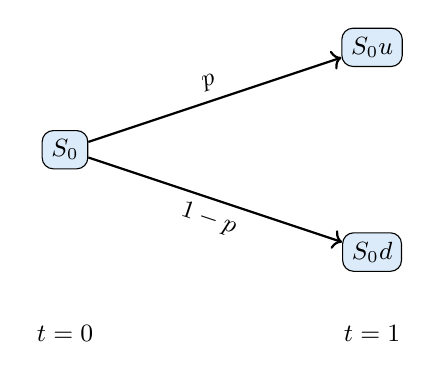
\begin{tikzpicture}[scale=1.3,every node/.style={font=\small}]
\node[draw,rounded corners,fill=lightblue] (S0) at (0,0) {$S_0$};
\node[draw,rounded corners,fill=lightblue] (Su) at (3,1) {$S_0 u$};
\node[draw,rounded corners,fill=lightblue] (Sd) at (3,-1) {$S_0 d$};
\draw[->,thick] (S0) -- (Su) node[midway,above,sloped] {\small $p$};
\draw[->,thick] (S0) -- (Sd) node[midway,below,sloped] {\small $1-p$};
\node at (0,-1.8) {$t=0$};
\node at (3,-1.8) {$t=1$};
\end{tikzpicture}
\caption{单步二叉树。}
\end{figure}

此外还有一个\textbf{无风险资产}（理解为银行存款）：放 1 块钱进去，下一时刻拿出 $1 + r$ 块（$r$ 是利率，比如 $r = 0.02$ 表示 2\% 利息）。无论涨跌，这个收益都是确定的。

我们要给一份看涨期权定价：到期收益是 $C_T = (S_1 - K)^+$。
记：
\[
C_u := (S_0 u - K)^+, \quad C_d := (S_0 d - K)^+.
\]
问题：今天这份合同 $C_0$ 应该是多少？

\subsection{第一种直觉（错的）}

最朴素的想法：算个期望，再贴现回来：
\[
C_0 \stackrel{?}{=} \frac{1}{1+r}\bigl[p\cdot C_u + (1-p)\cdot C_d\bigr]
\]
这\textbf{是错的}。原因下一节就清楚——这里有个让人惊讶的事实：\emph{真实概率 $p$ 不会出现在最终定价里}。

\subsection{无套利定价：复制组合}

正确的做法叫\emph{复制（replication）}。我们试图\textbf{用股票和银行存款，自己造一个跟这份期权一模一样的东西}。如果造得出来，那这份期权的价格就只能等于"造它的成本"，否则就有套利。

具体来说，今天买 $\Delta$ 股股票 + 借 $B$ 块钱（$B<0$ 表示存）。这个组合今天的价值是 $\Delta S_0 + B$。一个时刻后：
\begin{itemize}
    \item 股价涨时，组合值 $= \Delta S_0 u + B(1+r)$
    \item 股价跌时，组合值 $= \Delta S_0 d + B(1+r)$
\end{itemize}
要复制期权，要求两种情形下组合值都等于期权收益：
\begin{align*}
\Delta S_0 u + B(1+r) &= C_u \\
\Delta S_0 d + B(1+r) &= C_d
\end{align*}
两个方程两个未知数。两式相减：
\[
\boxed{\Delta = \frac{C_u - C_d}{S_0(u-d)}}
\]
这就是著名的"Delta 对冲比率"。代回任一方程解出 $B$：
\[
B = \frac{u C_d - d C_u}{(1+r)(u-d)}.
\]
所以期权的"造价"，也就是\textbf{今天的公平价格}是：
\[
C_0 = \Delta S_0 + B.
\]
代入整理（建议你自己推一遍），可以得到一个非常漂亮的形式：

\begin{idea}{单步二叉树定价公式}{single-step-formula}
\[
\boxed{C_0 = \frac{1}{1+r}\bigl[q\cdot C_u + (1-q)\cdot C_d\bigr]}, \quad
\boxed{q = \frac{(1+r) - d}{u - d}}
\]
其中 $q$ 称为\emph{风险中性概率（risk-neutral probability）}。
\end{idea}

\subsection{风险中性概率是什么？}

注意两件惊人的事：

\begin{enumerate}[leftmargin=*]
\item \textbf{真实概率 $p$ 完全没出现}。给期权定价不需要知道股票上涨的真实概率！这是因为我们是用\emph{复制}来定价——只要市场上能买卖股票和存款，造价就跟"为什么涨"无关。
\item \textbf{$q$ 长得像概率}。需要 $0 < q < 1$，等价于 $d < 1+r < u$，也就是说"涨"必须涨过无风险利率、"跌"必须跌破无风险利率（否则市场就有明显套利机会）。所以\emph{在一个无套利的市场里}，$q$ 自动落在 $(0,1)$ 中。
\end{enumerate}

把 $q$ 当成"假装的概率"，那么定价公式就读作：
\begin{center}
\itshape 期权今天的价格 = 在假装概率 $q$ 下，到期收益的期望，再用无风险利率贴现回今天。
\end{center}

为什么叫"风险中性"？因为在这套假装概率下，股票的期望收益率正好是无风险利率 $r$（请你算一下 $\E^\Q[S_1/S_0] = qu + (1-q)d = 1+r$）。这相当于把"愿意承担风险换更高收益"的偏好抽掉了。

\begin{exmp}{一个具体的数}{single-step-numerical}
设 $S_0 = 100$, $u = 1.2$, $d = 0.8$, $r = 0.02$, $K = 100$。看涨期权。
\begin{itemize}
\item $C_u = (120-100)^+ = 20$, $C_d = (80-100)^+ = 0$.
\item $q = (1.02 - 0.8)/(1.2-0.8) = 0.22/0.4 = 0.55$.
\item $C_0 = (0.55 \cdot 20 + 0.45 \cdot 0)/1.02 = 11/1.02 \approx 10.78$.
\end{itemize}
公平价格约 10.78 元。
\end{exmp}

% ==========================================================
\section{多步二叉树：从后往前算}
% ==========================================================

现实里时间不止"一步"。我们把 $[0, T]$ 切成 $N$ 个小段，每一段股价都按 $u$ 或 $d$ 跳一次。这就是\textbf{多步二叉树}。

\subsection{两步树长什么样}

\begin{figure}[h]
\centering
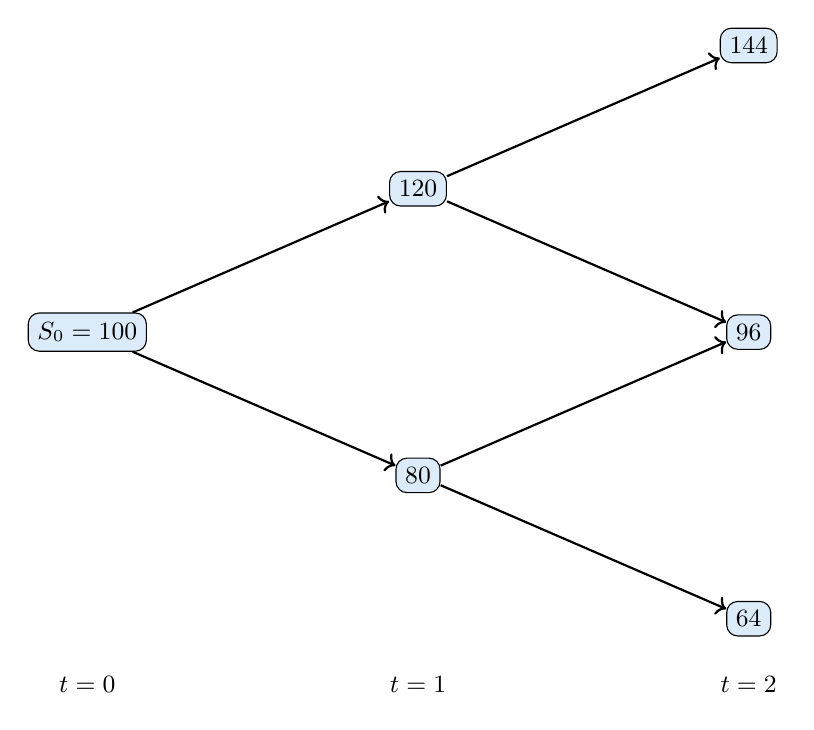
\begin{tikzpicture}[scale=1.4,every node/.style={font=\small}]
\node[draw,rounded corners,fill=lightblue] (S0)   at (0,0)   {$S_0=100$};
\node[draw,rounded corners,fill=lightblue] (Su)   at (3,1.3) {$120$};
\node[draw,rounded corners,fill=lightblue] (Sd)   at (3,-1.3) {$80$};
\node[draw,rounded corners,fill=lightblue] (Suu)  at (6,2.6) {$144$};
\node[draw,rounded corners,fill=lightblue] (Sud)  at (6,0)   {$96$};
\node[draw,rounded corners,fill=lightblue] (Sdd)  at (6,-2.6){$64$};
\draw[->,thick] (S0) -- (Su);
\draw[->,thick] (S0) -- (Sd);
\draw[->,thick] (Su) -- (Suu);
\draw[->,thick] (Su) -- (Sud);
\draw[->,thick] (Sd) -- (Sud);
\draw[->,thick] (Sd) -- (Sdd);
\node at (0,-3.2) {$t=0$};
\node at (3,-3.2) {$t=1$};
\node at (6,-3.2) {$t=2$};
\end{tikzpicture}
\caption{两步二叉树（$u=1.2, d=0.8$）。注意"涨跌"和"跌涨"汇合到同一个点（这叫\emph{重组树}，recombining tree）。}
\label{fig:two-step}
\end{figure}

\subsection{倒推（backward induction）}

定价的核心思想可以一句话讲清：

\begin{idea}{倒推原理}{backward-induction}
\itshape 在每一个节点，期权的价值等于"下一步两种可能性的（风险中性）期望，再贴现一步"。
\[
V_t(s) = \frac{1}{1+r}\bigl[q\, V_{t+1}(s \cdot u) + (1-q)\, V_{t+1}(s \cdot d)\bigr]
\]
我们从最右边（到期日）开始往左推，因为最右边的价值已经知道——就是收益函数 $g(S_T)$。
\end{idea}

\textbf{为什么倒推是对的？}因为多步树的每一个"局部"，本质上就是一个单步二叉树。在第 1 步那个节点上做复制对冲，仍然可以用单步公式。只不过我们不再是用现金对冲，而是用"下一步的期权价值"对冲。把每一步连起来就是动态对冲（dynamic hedging）。

\subsection{一个完整的数值例子（欧式看涨）}

继续用 $S_0=100, u=1.2, d=0.8, r=0.02, K=100$，到期日 $T = 2$ 步。$q = 0.55$。

\textbf{第一步：写出到期收益（在 $t=2$）}：
\[
C_{uu} = (144-100)^+ = 44, \quad C_{ud} = (96-100)^+ = 0, \quad C_{dd} = (64-100)^+ = 0.
\]

\textbf{第二步：倒推到 $t=1$}：
\begin{align*}
C_u &= \frac{1}{1.02}\bigl[0.55\cdot 44 + 0.45 \cdot 0\bigr] = \frac{24.2}{1.02} \approx 23.73 \\
C_d &= \frac{1}{1.02}\bigl[0.55\cdot 0 + 0.45 \cdot 0\bigr] = 0
\end{align*}

\textbf{第三步：倒推到 $t=0$}：
\[
C_0 = \frac{1}{1.02}\bigl[0.55 \cdot 23.73 + 0.45 \cdot 0\bigr] = \frac{13.05}{1.02} \approx 12.79
\]

\begin{figure}[h]
\centering
\begin{tikzpicture}[scale=1.4,every node/.style={font=\small}]
\node[draw,rounded corners,fill=lightblue] (S0)   at (0,0)   {$\substack{S=100\\C\approx 12.79}$};
\node[draw,rounded corners,fill=lightblue] (Su)   at (3,1.6) {$\substack{S=120\\C\approx 23.73}$};
\node[draw,rounded corners,fill=lightblue] (Sd)   at (3,-1.6) {$\substack{S=80\\C=0}$};
\node[draw,rounded corners,fill=lightgreen] (Suu)  at (6,3.2) {$\substack{S=144\\C=44}$};
\node[draw,rounded corners,fill=lightgreen] (Sud)  at (6,0)   {$\substack{S=96\\C=0}$};
\node[draw,rounded corners,fill=lightgreen] (Sdd)  at (6,-3.2){$\substack{S=64\\C=0}$};
\draw[->,thick] (S0) -- (Su);
\draw[->,thick] (S0) -- (Sd);
\draw[->,thick] (Su) -- (Suu);
\draw[->,thick] (Su) -- (Sud);
\draw[->,thick] (Sd) -- (Sud);
\draw[->,thick] (Sd) -- (Sdd);
\node at (0,-4.2) {$t=0$};
\node at (3,-4.2) {$t=1$};
\node at (6,-4.2) {$t=2$ (到期)};
\node[accentred] at (8.5, 3.2) {\small 已知};
\node[accentred] at (8.5, 0)   {\small 已知};
\node[accentred] at (8.5,-3.2) {\small 已知};
\draw[->,thick,accentred,dashed] (8.5,2) -- (8.5,-2) node[midway,right] {\small 倒推};
\end{tikzpicture}
\caption{欧式看涨期权的倒推。绿色是到期收益（已知），蓝色是倒推得到的价值。}
\end{figure}

\textbf{注意}：在这整个过程中，我们\emph{完全没有做任何决策}。每一步的"价值"是机械算出来的，因为欧式期权根本没有选择。

\subsection{再算一个：欧式看跌期权}

同样的树。看跌期权 $g(S) = (K - S)^+$：
\[
P_{uu} = 0, \quad P_{ud} = 4, \quad P_{dd} = 36.
\]
倒推：
\begin{align*}
P_u &= \frac{1}{1.02}[0.55 \cdot 0 + 0.45 \cdot 4] = \frac{1.8}{1.02} \approx 1.76 \\
P_d &= \frac{1}{1.02}[0.55 \cdot 4 + 0.45 \cdot 36] = \frac{2.2+16.2}{1.02} = \frac{18.4}{1.02} \approx 18.04 \\
P_0 &= \frac{1}{1.02}[0.55 \cdot 1.76 + 0.45 \cdot 18.04] = \frac{0.968+8.118}{1.02} \approx 8.91
\end{align*}
所以这份欧式看跌期权今天值 $\approx 8.91$ 元。\textbf{请记住 8.91 这个数}——下一节会跟它对比。

% ==========================================================
\section{美式期权：决策的出现}\label{sec:american}
% ==========================================================

现在我们换成\textbf{美式看跌}期权。规则只多了一条：\emph{你可以在 $t=0, 1, 2$ 的任何时候选择立刻行权}（行权了立刻拿钱，合同失效）。

\subsection{为什么这会改变结果？}

继续看上面那个例子。考虑 $t=1$ 时股价跌到了 80 的情形。

\begin{itemize}[leftmargin=*]
    \item \textbf{现在马上行权}的话，立即拿到 $(100 - 80)^+ = 20$ 元。
    \item \textbf{再等一步}的话，相当于持有一个剩一步的欧式看跌期权，刚才算过了，价值约 18.04 元。
\end{itemize}

\textbf{20 > 18.04}！立刻行权赚得更多。所以这个节点上的最优决策是：\textbf{马上行权}。

这就是欧式和美式的根本区别：美式期权的持有者，在每一个节点都要做一个\emph{二选一}：
\[
\boxed{\text{停下来（行权）} \quad \text{vs} \quad \text{继续持有}}
\]

\subsection{美式期权的 Bellman 方程}

把上面这个直觉写成数学：

\begin{idea}{美式期权的递归公式}{american-bellman}
设 $V_t(s)$ 是美式期权在时刻 $t$、股价为 $s$ 时的价值，则：
\[
\boxed{
V_t(s) = \max\Big\{\underbrace{g(s)}_{\text{马上行权}}, \quad \underbrace{\tfrac{1}{1+r}\bigl[q V_{t+1}(su) + (1-q) V_{t+1}(sd)\bigr]}_{\text{继续持有}}\Big\}
}
\]
边界条件 $V_T(s) = g(s)$（到期必须行权，没法再等了）。
\end{idea}

\begin{itemize}[leftmargin=*]
    \item 第一项 $g(s)$ 叫\emph{内在价值（intrinsic value）}或\emph{行权价值（exercise value）}。
    \item 第二项叫\emph{延续价值（continuation value）}。
    \item 取 $\max$ 就是"两条路里挑收益高的那条"。
\end{itemize}

注意，欧式期权那个公式里只有第二项，没有 $\max$，因为欧式根本不允许提前行权——它的"决策空间"只有一个动作（"等"），所以不用挑。

\subsection{对前面的例子重算一遍}

同样的树，同样的 $q = 0.55$，看跌期权 $g(s) = (100 - s)^+$。

\textbf{在 $t = 2$（到期）}：
\[
V_{uu} = 0, \quad V_{ud} = 4, \quad V_{dd} = 36 \quad (\text{和欧式一样})
\]

\textbf{在 $t = 1$，上节点（$s = 120$）}：
\begin{itemize}
    \item 行权值：$g(120) = 0$
    \item 延续值：$\frac{1}{1.02}[0.55 \cdot 0 + 0.45 \cdot 4] \approx 1.76$
    \item $V_u = \max(0, 1.76) = 1.76$，决策：\textcolor{accentgreen}{\bfseries 继续持有}
\end{itemize}

\textbf{在 $t = 1$，下节点（$s = 80$）}：
\begin{itemize}
    \item 行权值：$g(80) = 20$
    \item 延续值：$\frac{1}{1.02}[0.55 \cdot 4 + 0.45 \cdot 36] \approx 18.04$
    \item $V_d = \max(20, 18.04) = \mathbf{20}$，决策：\textcolor{accentred}{\bfseries 马上行权！}
\end{itemize}

\textbf{在 $t = 0$（$s = 100$）}：
\begin{itemize}
    \item 行权值：$g(100) = 0$
    \item 延续值：$\frac{1}{1.02}[0.55 \cdot 1.76 + 0.45 \cdot 20] = \frac{0.968 + 9.0}{1.02} \approx 9.77$
    \item $V_0 = \max(0, 9.77) = 9.77$，决策：\textcolor{accentgreen}{\bfseries 继续持有}
\end{itemize}

\begin{figure}[h]
\centering
\begin{tikzpicture}[scale=1.4,every node/.style={font=\small}]
\node[draw,rounded corners,fill=lightblue] (S0)   at (0,0)   {$\substack{S=100\\V\approx 9.77\\\text{\scriptsize 持}}$};
\node[draw,rounded corners,fill=lightblue] (Su)   at (3,1.7) {$\substack{S=120\\V\approx 1.76\\\text{\scriptsize 持}}$};
\node[draw,rounded corners,fill=lightred] (Sd)   at (3,-1.7) {$\substack{S=80\\V=\mathbf{20}\\\text{\scriptsize \bfseries 行权!}}$};
\node[draw,rounded corners,fill=lightgreen] (Suu)  at (6,3.4) {$\substack{S=144\\V=0}$};
\node[draw,rounded corners,fill=lightgreen] (Sud)  at (6,0)   {$\substack{S=96\\V=4}$};
\node[draw,rounded corners,fill=lightgreen] (Sdd)  at (6,-3.4){$\substack{S=64\\V=36}$};
\draw[->,thick] (S0) -- (Su);
\draw[->,thick] (S0) -- (Sd);
\draw[->,thick] (Su) -- (Suu);
\draw[->,thick] (Su) -- (Sud);
\draw[->,thick,dashed,accentred,line width=1pt] (Sd) -- (Sud);
\draw[->,thick,dashed,accentred,line width=1pt] (Sd) -- (Sdd);
\node at (0,-4.4) {$t=0$};
\node at (3,-4.4) {$t=1$};
\node at (6,-4.4) {$t=2$};
\end{tikzpicture}
\caption{美式看跌期权。红色节点表示最优决策是"立即行权"，那条路径上的后续节点（虚线）实际上不会发生。$V_0 \approx 9.77 > 8.91$（欧式价格），多出来的 $0.86$ 正是"提前行权权利"带来的额外价值。}
\end{figure}

\subsection{两个深刻的观察}

\begin{enumerate}[leftmargin=*]
\item \textbf{美式期权 $\geq$ 欧式期权}：因为美式允许更多行权方式，欧式是它的一个特例（"我就一直等到 $T$"）。多出来那一点价值就是"提前行权权利"的价值，叫做\emph{early exercise premium}。这里它是 $9.77 - 8.91 = 0.86$。
\item \textbf{最优行权区域}：把最优决策为"立刻行权"的所有 $(t, s)$ 节点圈起来，叫\emph{停止区域（stopping region）}。它的补集叫\emph{继续区域（continuation region）}。两者之间的边界叫\emph{最优行权边界（optimal exercise boundary）}。
    在我们的小例子里：最优行权区域 = $\{(t=1, s=80)\} \cup \{t=2 \text{ 所有节点}\}$。
\end{enumerate}

\begin{idea}{决策的本质}{decision-essence}
\itshape 美式期权定价中，"提前行权"和"继续持有"构成了一个二元的动作空间。每个节点选择哪个动作，不是拍脑袋的，而是由 $\max$ 算出来的——挑那条让长期价值最大的路。这就是\textbf{最优决策}问题的雏形：在每一个状态下，从可选动作里挑一个，使未来累积价值最大。
\end{idea}

% ==========================================================
\section{抽象：把决策过程的语言提炼出来}
% ==========================================================

到这里为止，我们一直在讲期权。但仔细看美式期权那个 $\max\{\ldots\}$ 的结构，里面其实没有任何特别"金融"的东西。我们把它抽离出来。

\subsection{四个核心要素}

把美式期权的定价过程改写成更一般的语言：

\medskip
\noindent
\begin{tabular}{@{}p{3.5cm}p{4.5cm}p{6.5cm}@{}}
\toprule
\textbf{抽象概念} & \textbf{符号} & \textbf{在美式期权里的具体对应} \\
\midrule
状态 (state) & $s_t$ & 当前股价（和当前时刻）\\
动作 (action) & $a_t$ & 行权 / 继续持有 \\
奖励 (reward) & $r(s, a)$ & 行权时拿到 $g(s)$，继续时拿 0 \\
转移 (transition) & $P(s' \mid s, a)$ & 继续时按 $q, 1-q$ 跳到 $su$ 或 $sd$；行权后进入"已结束"状态 \\
折现因子 (discount) & $\gamma$ & $1/(1+r)$ \\
\bottomrule
\end{tabular}
\medskip

这就是\textbf{马尔可夫决策过程（Markov Decision Process, MDP）}的全部要素：$(S, A, P, r, \gamma)$。

\begin{defn}{马尔可夫决策过程}{mdp}
一个 MDP 包含五元组 $(\mathcal{S}, \mathcal{A}, P, r, \gamma)$：
\begin{itemize}
    \item $\mathcal{S}$：状态空间
    \item $\mathcal{A}$：动作空间
    \item $P(s'\mid s,a)$：从 $s$ 采取动作 $a$ 后转移到 $s'$ 的概率
    \item $r(s,a)$：即时奖励
    \item $\gamma \in [0,1)$：折现因子
\end{itemize}
"马尔可夫"是指：下一步只取决于当前状态和动作，不取决于历史路径——美式期权恰好满足，因为期权价值只跟当前股价有关（不管之前走的是涨涨跌还是跌涨涨）。
\end{defn}

\subsection{价值函数与最优策略}

\begin{defn}{策略与价值函数}{policy-value}
\textbf{策略（policy）}：一个函数 $\pi: \mathcal{S} \to \mathcal{A}$，告诉你在每个状态选哪个动作。在美式期权里，策略就是"哪些节点行权、哪些节点继续"。

\textbf{状态值函数（state-value function）}：
\[
V^\pi(s) := \E\Big[\sum_{t=0}^{\infty} \gamma^t r(s_t, \pi(s_t)) \,\Big|\, s_0 = s\Big]
\]
意思是：从状态 $s$ 出发，按策略 $\pi$ 一直走下去，未来奖励的折现累加（取期望，因为转移有随机性）。

\textbf{最优值函数}：$V^*(s) := \max_\pi V^\pi(s)$。

\textbf{最优策略}：达到 $V^*$ 的那个 $\pi$，记 $\pi^*$。
\end{defn}

% ==========================================================
\section{这就是强化学习：Bellman 方程}
% ==========================================================

下面这个方程是这门课的"主定理"。

\subsection{最优 Bellman 方程}

\begin{idea}{Bellman 最优方程}{bellman-optimality}
最优值函数 $V^*$ 满足：
\[
\boxed{
V^*(s) = \max_{a \in \mathcal{A}}\Big\{r(s,a) + \gamma\, \E_{s'\sim P(\cdot\mid s,a)}[V^*(s')]\Big\}
}
\]
即：在每个状态，挑那个让"即时奖励 + 折现后未来最优价值期望"最大的动作。
\end{idea}

把它代到美式期权的设置里：动作只有"行权"和"继续"两个。

\begin{itemize}[leftmargin=*]
    \item 选"行权"：$r = g(s)$，之后游戏结束（$V^*$ 为 0）。所以这条分支的值 $= g(s)$。
    \item 选"继续"：$r = 0$，转移到 $s' \in \{su, sd\}$，概率 $q, 1-q$。这条分支的值 $= \gamma \E[V^*(s')] = \frac{1}{1+r}[q V^*(su) + (1-q) V^*(sd)]$。
\end{itemize}

把这两个分支拿 $\max$，立刻得到第~\ref{sec:american}~节我们写过的美式期权公式：
\[
V^*_t(s) = \max\Big\{g(s),\ \tfrac{1}{1+r}\bigl[q V^*_{t+1}(su) + (1-q) V^*_{t+1}(sd)\bigr]\Big\}
\]
\textbf{完全一样}。两者只是符号不同。

\begin{idea}{重点回顾}{key-takeaway}
\itshape\large
美式期权的倒推 = MDP 的 Bellman 方程 = 强化学习的核心。

\smallskip
你刚才学会的"倒推 + 取 max"，就是强化学习里所谓的\textbf{动态规划（dynamic programming）}和\textbf{值迭代（value iteration）}的原型。
\end{idea}

\subsection{为什么这叫"强化学习"还差一步？}

我们目前讲的所有内容，更准确地说叫\textbf{已知模型的最优控制（optimal control with known model）}。因为我们假定：
\begin{itemize}
    \item 转移概率 $q$ 已知（从无套利推出来的）；
    \item 奖励函数 $g(\cdot)$ 已知；
    \item 状态空间显式可枚举（二叉树的所有节点）。
\end{itemize}
真正的"强化学习"问题是：\textbf{这些都未知或者大到无法枚举}，智能体只能通过\emph{和环境交互、观察样本}来学习。

但是！只要你理解了倒推这一步——
\[
V(s) \leftarrow \max_a \Big\{r(s,a) + \gamma\, \E[V(s')]\Big\}
\]
你就理解了 RL 里所有主要算法的内核。它们都在做同一件事，只是处理"未知"和"大"的方式不同：

\begin{itemize}[leftmargin=*]
    \item \textbf{Q-learning}：把 $V$ 换成 $Q(s,a)$，用样本估计期望，不需要知道 $P$。
    \item \textbf{Deep Q-Network (DQN)}：用神经网络逼近 $Q$，处理状态空间太大无法枚举的情况。
    \item \textbf{Policy Gradient}：直接对 $\pi$ 求导，跳过 $V$ 的显式计算。
    \item \textbf{Actor-Critic}：$V$（critic）和 $\pi$（actor）一起学。
\end{itemize}

事实上，金融工程界还在用"美式期权"这个具体问题来检验 RL 算法。Longstaff–Schwartz 在 2001 年提出的 "最小二乘蒙特卡洛" 方法——本质上就是用样本+回归来逼近"延续价值"——是早于现代 RL 文献的一个例子，今天我们会把它叫做"用线性函数逼近的拟合 Q 迭代（fitted Q-iteration with linear function approximation）"。

% ==========================================================
\section{几个延伸思考}
% ==========================================================

\subsection{思考一：为什么"假装概率" $q$ 在 RL 里不出现？}

在金融里我们用风险中性概率 $q$ 而不是真实概率 $p$，是因为我们要"无套利定价"——价格是\emph{交换价值}的镜像，必须把风险偏好剥离掉。

在 RL 里，转移概率就是真实的环境动力学，没有"风险中性测度"这个东西。但是！如果你要做的是\emph{风险敏感}的 RL（比如最小化 CVaR 而不是期望），那 \emph{风险测度} 又会作为某种"扭曲的概率"出现——这跟金融里的风险中性测度是同一套数学（凸对偶、变分表示）。这是为什么 risk-sensitive RL 和金融数学共享大量工具。

\subsection{思考二：连续时间在哪里？}

我们这里讲的是\emph{离散时间} 二叉树。如果你把每一步的 $\Delta t \to 0$，并且让 $u, d$ 选成 $u = e^{\sigma\sqrt{\Delta t}}, d = e^{-\sigma\sqrt{\Delta t}}$（Cox-Ross-Rubinstein 选法），二叉树会收敛到\emph{Black-Scholes 模型}——著名的 BSM 偏微分方程：
\[
\frac{\partial V}{\partial t} + \frac{1}{2}\sigma^2 s^2 \frac{\partial^2 V}{\partial s^2} + rs\frac{\partial V}{\partial s} - rV = 0
\]
正是 Bellman 方程的连续时间极限（叫 Hamilton–Jacobi–Bellman 方程，HJB）。所以 \emph{二叉树 $\to$ Black-Scholes PDE} 与 \emph{Bellman $\to$ HJB} 是同一种"离散到连续"的过程。

\subsection{思考三：决策的"代价"在哪里？}

注意我们的美式期权例子里，"动作"本身不消耗任何成本：行权就直接拿钱，继续就直接跳到下一步。现实的 RL 任务里，几乎总有动作的代价——能耗、磨损、机会成本。在金融里这对应于\emph{交易成本、市场冲击、库存约束}，把这些加进来，期权定价立刻变成一个真正的 RL 问题（无解析解、需要数值/学习方法），这就是近年来的"deep hedging"路线。

% ==========================================================
\section*{进一步阅读}
% ==========================================================
\addcontentsline{toc}{section}{进一步阅读}

\begin{itemize}[leftmargin=*]
    \item Hull, J. C. \emph{Options, Futures, and Other Derivatives}. 入门金融衍生品的经典教材。第 13 章详细讲二叉树。
    \item Shreve, S. \emph{Stochastic Calculus for Finance I: The Binomial Asset Pricing Model}. 把二叉树讲到数学的极致，是最适合数学/计算背景学生的金融入门。
    \item Sutton, R., Barto, A. \emph{Reinforcement Learning: An Introduction}. RL 的标准教材，前 4 章正好与本讲义内容对应。
    \item Longstaff, F., Schwartz, E. (2001). "Valuing American Options by Simulation: A Simple Least-Squares Approach." \emph{Review of Financial Studies}, 14(1), 113--147. 美式期权与回归的桥梁，是 RL 视角下最经典的金融论文之一。
\end{itemize}

\end{document}
